\sect{5. C\'omo se juega}

Eres un luchador de kung-fu que se abre paso por cinco fases, desde la sala de un templo hasta un paso de monta\~na.
Cada fase tiene varios pisos: sube con \key{$\uparrow$}, baja con \key{$\downarrow$}. En todas las fases el plan es el mismo:

\begin{enumerate}
\item \textbf{Derrota a los 21 enemigos} que salen de las dos puertas y de los lados. T\'umbalos a patadas; la patada voladora da m\'as puntos.
\item Cuando cae el \'ultimo de la oleada aparece el \textbf{jefe} de la fase. Golp\'ealo \textbf{cinco veces} para vencerlo.
\item Vence al jefe y la fase termina: se cuenta tu bonus \textbf{GUTS!} y empieza el siguiente \texttt{STEP}.
\end{enumerate}

Tras la quinta fase el juego vuelve a la primera, con enemigos m\'as r\'apidos y agresivos. A partir de la segunda vuelta, un \textbf{p\'ajaro} cruza la fase de vez en cuando y \textbf{suelta una piedra}: ap\'artate.

Algunos enemigos llevan una \textbf{bola de poder}. Derriba al portador para conseguir un arma especial durante un rato.

Cada fase tiene l\'imite de tiempo. Cuando queda poco aparece el cartel \texttt{HURRY UP}, y si se agota pierdes una vida (\texttt{TIME OVER}). Cuantos m\'as enemigos hay que vencer, m\'as tiempo te dan.

% ==================================================================
\sect{6. El marcador (HUD)}

\begin{figure}[H]
\centering
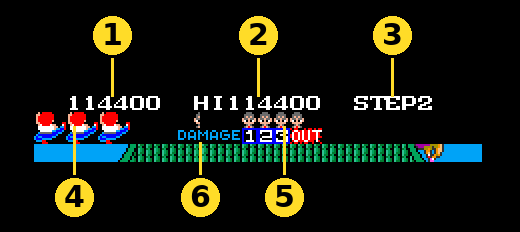
\includegraphics[width=\textwidth]{img/hud.png}
\caption{El marcador, en la parte superior de la pantalla.}
\end{figure}

\begin{tabularx}{\textwidth}{@{}cp{3.1cm}X@{}}
\toprule
\textbf{\tNo} & \textbf{\tElement} & \textbf{\tTellsYou}\\
\midrule
1 & Puntuaci\'on & Tu puntuaci\'on.\\
2 & R\'ecord & La mejor puntuaci\'on de la tabla de r\'ecords.\\
3 & Fase & \texttt{STEP} y el n\'umero de fase, contando las vueltas (tras la quinta fase viene \texttt{STEP 6}).\\
4 & Vidas & Un icono por cada vida de reserva; con cinco o m\'as muestra un icono y el n\'umero.\\
5 & Enemigos que quedan & Cada cabecita equivale a tres enemigos por vencer en la oleada; se acorta a medida que ganas.\\
6 & Da\~no & \texttt{DAMAGE 1 2 3 OUT}: cada golpe enciende un n\'umero m\'as y el actual parpadea. El cuarto golpe, \texttt{OUT}, cuesta una vida.\\
\bottomrule
\end{tabularx}

% ==================================================================
\sect{7. Puntuaci\'on y vidas}

\begin{center}
\begin{tabular}{@{}lr@{}}
\toprule
\textbf{Acci\'on} & \textbf{Puntos}\\
\midrule
Patada a un enemigo & 200\\
Patada voladora & 500\\
Combo (segundo K.O. seguido y r\'apido) & 1000\\
Hacer aparecer el objeto de bonus & 500\\
Bonus GUTS!, por cada nivel de da\~no sin usar & 1000\\
\bottomrule
\end{tabular}
\end{center}

\begin{itemize}
\item Empiezas con \textbf{3 vidas}.
\item Ganas una \textbf{vida extra a los 40\,000 puntos y despu\'es cada 80\,000}.
\item La dificultad es la que eliges en la pantalla de t\'itulo, \textbf{dif\'icil} (\key{1}) o \textbf{medio} (\key{2}), y aumenta con cada fase que superas.
\item Tras \texttt{GAME OVER}, las ocho mejores puntuaciones quedan en la \textbf{tabla de r\'ecords}, con tus tres iniciales: cambia la letra con izquierda y derecha, y patea para aceptarla. La tabla empieza con los nombres \texttt{MSX}, \texttt{BTV}, \texttt{DI}, \texttt{HLT}, \texttt{KON} y \texttt{AMI}.
\end{itemize}

\begin{figure}[H]
\centering
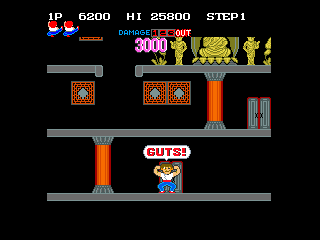
\includegraphics[width=0.48\textwidth]{../img/guts.png}\hfill
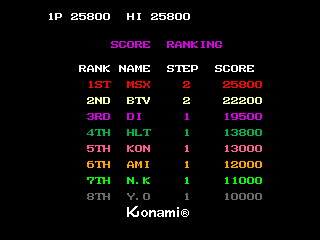
\includegraphics[width=0.48\textwidth]{../img/ranking.png}
\caption{Izquierda: el bonus \texttt{GUTS!} al final de una fase. Derecha: la tabla de r\'ecords.}
\end{figure}

% ==================================================================
\sect{8. Consejos}

\begin{itemize}
\item No te quedes quieto: los enemigos te rodean. Pelea con la espalda contra una pared o una puerta solo si tienes espacio para retroceder.
\item La patada tiene poco alcance. Deja que el enemigo se acerque y patea cuando llegue.
\item La patada voladora da 500 puntos frente a 200 de la patada normal y salva huecos, pero te deja expuesto mientras est\'as en el aire.
\item Usa arriba y abajo para cambiar de piso, y f\'ijate en los enemigos que esperan en el piso al que vas.
\item Mant\'en bajo tu da\~no: cada nivel que no uses vale \textbf{1000 puntos} al terminar la fase.
\item Mira los iconos de cabeza: cuando quedan pocos, el jefe est\'a cerca.
\item Desde la segunda vuelta, mira hacia arriba cuando oigas al p\'ajaro.
\item Vigila siempre el tiempo: con \texttt{HURRY UP} en pantalla, ve directo a por los enemigos que quedan.
\end{itemize}
